\documentclass[14pt,a4paper]{article}
%\renewcommand{\baselinestretch}{1.5}
\linespread{1.3}
\usepackage[T2A]{fontenc} % Поддержка русских букв
\usepackage[utf8]{inputenc} 
\usepackage[english,russian]{babel}  
\bibliographystyle{unsrt}


\usepackage{graphicx}
\graphicspath{{imageWiMAX/}}
 
\begin{document}
\renewcommand\refname{Литература}
\thispagestyle{empty}

\begin{center}
\textbf{САНКТ-ПЕТЕРБУРГСКИЙ НАЦИОНАЛЬНЫЙ ИССЛЕДОВАТЕЛЬСКИЙ УНИВЕРСИТЕТ ИНФОРМАЦИОННЫХ ТЕХНОЛОГИЙ, 
МЕХАНИКИ И ОПТИКИ}

Факультет Компьютерных технологий и управления\\
Кафедра вычислительной техники
\end{center}
\vspace{2.5cm}

\begin{center}
\textbf{ОТЧЕТ}
\\
\textbf{о практике}

Исследование сетевых технологий с помощью имитационного моделирования
\end{center}

\vspace{2.5cm}

\begin{flushright}
\textbf{Студент}\\
Елькин А. А. группа 3105

\textbf{Руководитель практики}\\
Соснин В. В. доцент
\end{flushright}
\vspace{6cm}
\begin{center}
2014 год
\end{center}
%+++++++++++++++++++++++++++++++++++++++++++++++++++++++++++++++++++++++++++++++++++++++++++++++++++
%+++++++++++++++++++++++++++++++++++++++++++++++++++++++++++++++++++++++++++++++++++++++++++++++++++
%+++++++++++++++++++++++++++++++++++++++++++++++++++++++++++++++++++++++++++++++++++++++++++++++++++
%+++++++++++++++++++++++++++++++++++++++++++++++++++++++++++++++++++++++++++++++++++++++++++++++++++
%+++++++++++++++++++++++++++++++++++++++++++++++++++++++++++++++++++++++++++++++++++++++++++++++++++
\newpage
\tableofcontents
%+++++++++++++++++++++++++++++++++++++++++++++++++++++++++++++++++++++++++++++++++++++++++++++++++++
%+++++++++++++++++++++++++++++++++++++++++++++++++++++++++++++++++++++++++++++++++++++++++++++++++++
%+++++++++++++++++++++++++++++++++++++++++++++++++++++++++++++++++++++++++++++++++++++++++++++++++++
%+++++++++++++++++++++++++++++++++++++++++++++++++++++++++++++++++++++++++++++++++++++++++++++++++++
%+++++++++++++++++++++++++++++++++++++++++++++++++++++++++++++++++++++++++++++++++++++++++++++++++++
\newpage
\section{Система компьютерной верстки \TeX(\LaTeX)}
\subsection{\TeX}
\subsubsection{История \TeX}
\TeX{} \cite{wikiTeX:website} ~--- система компьютерной верстки, разработанная
Дональдом Кнутом, которая предназанчена для компьютерной верстки текста и математических формул. Кнут
начал разрабатывать систему в 1977 году, и первая версия \TeX{} вышла 1979
года. В 1982 году вышла заново переписанная версия \TeX'а, которой было дано
название TeX82. И с версии \TeX{} 3.0, которая получила лучшую поддержку
8-битных символов и различных языков, используеться нумирация: каждое обновление
добавляет в конец номера версии десятичную цифру так, что бы она приблежалась к
числу \begin{math} \pi \end{math}.

\subsubsection{Особенности \TeX}
В \TeX{} пользователь пишет тескст и задает лишь струкуту самого текста, а система
сама формирует документ на основе выбранного шаблона. Для задания структуры
используеться собственный язык разметки \TeX'а, все это содержиться в фалье с
расширением .tor, и \TeX{} транслирует в файл .dvi.

\TeX{} можно использовать для создания разных видов докуметов: книги, статьи,
отчеты, письма и др.

\subsection{\LaTeX}
\LaTeX{} \cite{wikiLaTeX:website}~--- макропакет компьютерной верстки \TeX{}. Он
не добаляет возможности в \TeX{}, а лишь позволяет автоматизировать задачи набора текста(умерация
разделов и формул, перекресные ссылки, размещение таблиц и т. п.). Первую версию
выпустил Лесли Лэмпортв 1984 году. В 1994 году была выпущена вторая версия
\LaTeX -- \LaTeXe{}, которая являеться текущей по сей день.

\subsection{Достоинства и недостатки \cite{Lvovskii}}
Среди достоинств можно выделить:
\begin{itemize}
\item{}Автор может не вникать в детали оформления документа, ему лишь надо
задать логическую структуру текста.
\item{}высокое качество и гибкость верстки абзацев и математических формул.
\item{}\TeX{} не требует большой вычеслительной мощности.
\item{}Система работает на большенства платформах.
\end{itemize}
Среди недостатков можно выделить:
\begin{itemize}
\item{}Исходный текст не будет выглядеть так же как при печати.
\item{}Создание нового макета документа очень трудоемкая задача.
\item{}\TeX{} плохо приспособлен для верстки страниц со сложным взаимодействие текста
и графиков.
\end{itemize}

\subsection{Список выбранного ПО}
Для написания отчета по практике был выбра ряд программного обеспечения:
\begin{enumerate}
\item Сборка \TeX'а MacTeX(http://tug.org/mactex/), включающий pdfLaTeX, который
выдает документ с расширение pdf.
\item IDE Eclipse(https://www.eclipse.org/) с расширением
TeXlipse(http://texlipse.sourceforge.net/), позволяющие удобно редактировать
документ.
\end{enumerate}
%+++++++++++++++++++++++++++++++++++++++++++++++++++++++++++++++++++++++++++++++++++++++++++++++++++
%+++++++++++++++++++++++++++++++++++++++++++++++++++++++++++++++++++++++++++++++++++++++++++++++++++
%+++++++++++++++++++++++++++++++++++++++++++++++++++++++++++++++++++++++++++++++++++++++++++++++++++
%+++++++++++++++++++++++++++++++++++++++++++++++++++++++++++++++++++++++++++++++++++++++++++++++++++
%+++++++++++++++++++++++++++++++++++++++++++++++++++++++++++++++++++++++++++++++++++++++++++++++++++
\newpage
\section{Система контроля верси Git}
\subsection{История Git}
Git \cite{wikiGit:website}~--- распределенная система контроля версиями.
Причиной создания Git послужило ухудшение отношейний между сообществом разработчиков Linux и компанией
разработавшей BitKeeper, используемым сообществом с 2002 года для разработки
Linux. Создателем проекта был Линус Торвальдс, и на сегодняшний день
поддердживаеться Джунио Хамано.
\subsection{Особенности Git}
В отличии от дугих СКВ Git не хранит изминения файлов, а сохраняет слепок файла
как она выгляид в данный момент, при чем, если файл не был изменен, он делает
ссылку на ранюю сохраненную версию файла. Так же большенство опраций с файлами
происходит локально, то есть для просмотра истории изменения проекта, создания
коммита можно не иметь доступа к Сети.

Git следит за целостностью данных, он вычисляет контрольную сумму(SHA-1 хеш),
которая становиться индексом данного файла. Данная система не позваляет изменять
содержимое файлов или каталога.
\subsection{Git-команды\cite{web:ProGit}}
\begin{enumerate}
  \item git help предаставляет список команд. Если использовать git
  --help <имя команды> даст справку об определенной команде.
  \item git init создает каталог .git со всей необходимой информацией о
  репозитории.
  \item git clone клонирует существующий репозиторий
  \item git remote отображает уже подключенные репозитории
  \item git remote add добавляет удаленный репозиторий
  \item git remote rm удаляет ссылку на репозиторий
  \item git add индексирует измененных файлом 
  \item git commit фиксирует измененные файлы
  \item git rm удаляет файлы
\end{enumerate}
Примеры ипользования приведенных команды находяться в каталоге "примеры Git
команд"
%+++++++++++++++++++++++++++++++++++++++++++++++++++++++++++++++++++++++++++++++++++++++++++++++++++
%+++++++++++++++++++++++++++++++++++++++++++++++++++++++++++++++++++++++++++++++++++++++++++++++++++
%+++++++++++++++++++++++++++++++++++++++++++++++++++++++++++++++++++++++++++++++++++++++++++++++++++
%+++++++++++++++++++++++++++++++++++++++++++++++++++++++++++++++++++++++++++++++++++++++++++++++++++
%+++++++++++++++++++++++++++++++++++++++++++++++++++++++++++++++++++++++++++++++++++++++++++++++++++
\newpage
\section{WiMAX}
WiMAX\cite{wikiWiMAX:website} ~--- телекоммуникационная технология,
предоставляющая универсальный беспроводной связи на большие расстояния для
разных устройств. Сеть WiMAX представляет собой совокунпность беспроводного
сегмента, который описываеться в стандарте IEEE 802.16, и базового сегмента, определенный
спецификациями WiMAX-форума\cite{WiMAXForum:website}.
\subsection{История WiMAX}
В декабре 2001 года была принята первая версия стандарта IEEE 802.16, который
описывал организацию широкоплосной беспроводной связи. Стандарт предусматривал 
скорость передачи информации 32-134 Мбит/с на расстояние в 2-5 км в радиоканалах
шириной 20, 25 и 28 МГц.

Из-за того, что была необходимо построение беспроводной сети только в зоне
прямой видимости, стандарт не получил широкого распространения. По этому в
январе 2003 года был принято расширение 802.15a, который изменял используемые
частоты на ча стоты в диапозоне от 2 до 11 ГГц. Это расширение должно было
обеспечивать скорость передачи информации 1-75 Мбит/с на теоретическое возможное
растояние 50км(в основном 6-9 км).

Стандарт IEEE 802.16e приняли в 2005 году. Он поддерживает мобильных абонентов и
систему роуминга между сетями различных беспроводных стандартов. 802.16e
позволял без разрыва сеанса переключаться между стандартами 802.11 и 802.16.

\subsection{Структура\cite{PathWiMAX} WiMAX}
Сеть состоит из двух основных подсистем: Access Service Network(Сеть доступа) и
Connectivity Service Network(Сеть обеспечения услуг).

\begin{center}
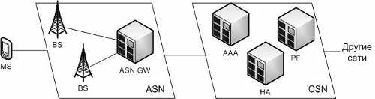
\includegraphics[scale=0.75]{WIMAX}\\
Структура сети WIMAX
\end{center}

CSN определяеться как набор функций для
абонента сети:
\begin{itemize}
\item{}Распределение адрессов между абонентами
\item{}Доступ к сети Интернет
\item{}Контроль доступа абонентов в сети
\item{}Биллинг и межаператорское взаимодествие
\item{}Обеспечение сервисов WiMAX
\item{}Обеспечение аутенфикации, авторизации и аудита соединения
\end{itemize}

CNS пренадлежит оператору WiMAX, которому пренадлежат маршрутезаторы, серверы
для авторизации, вутенфикации и аудита, базы данных пользователей, устройства
преобразования сигнала.

ASN ~--- набор сетевых элементов, организующие доступ в WiMAX сеть, выполняющие
функции:
\begin{itemize}
\item{}Доступ абонентов сеть по радиосвязи
\item{}Передача сообщений между CSN и абонентом для обеспечения аутенфикации,
авторизации и аудита соединения
\item{}Правление радиоресурсами
\item{}Поиск абонента в сети
\item{}Мобильность абонента
\end{itemize}

ASN представляет собой множество базовых станций, которые предоставляю доступ по
радиосвязи по стандарту IEEE 802.16, и шлюза, предназначенного для объединения
трафика от базовых станций и передачи его в CNS. ASN обязательно включает одну
базовую станцию и один ASN-шлюз. Одной ASN могут пользоваться несколько
провайдеров WiMAX(каждый со своей CNS).

Но так же не стоит забывать о большом количестве абонентов(мобильных станций). В
качестве их могут быть мобтльные телефены, смартфоны, ноутбуки и другие
устройства со встроенным или внешним адаптером.
%+++++++++++++++++++++++++++++++++++++++++++++++++++++++++++++++++++++++++++++++++++++++++++++++++++
%+++++++++++++++++++++++++++++++++++++++++++++++++++++++++++++++++++++++++++++++++++++++++++++++++++
%+++++++++++++++++++++++++++++++++++++++++++++++++++++++++++++++++++++++++++++++++++++++++++++++++++
%+++++++++++++++++++++++++++++++++++++++++++++++++++++++++++++++++++++++++++++++++++++++++++++++++++
%+++++++++++++++++++++++++++++++++++++++++++++++++++++++++++++++++++++++++++++++++++++++++++++++++++
\newpage
\section{Выполнение задания по теме}
\subsection{ПО ns-3}
ns-3\cite{ns3W:website} ~--- это дискретно-событийный симулятор сети, свободно
распространяющийся под лицензией  GNU GPLv2 license. Основное использование ns-3 фокусируебться на
беспровобном или IP моделирование, которое включаетодели для Wi-Fi, WiMAX и LTE.
\subsubsection{Установка ns-3}
Для установки потребовалось:
Mercurial(hg)(http://aragost.com/mercurial/)-система контроля версии.
GNU Compiler Collection(http://gcc.gnu.org/).

Для начала нужно было было клонировать репозиторий, в котором размещались
скрипты для скачивания и установки ns-3(скриншот downloadScripts.jpg).
\begin{quote}
hg clone http://code.nsnam.org/ns-3-allinone
\end{quote}
\vspace{0.75cm}
Затем запускаелся скрипт для загрузки исходных файлов ns-3(скришот
downloadFileToInstall.jpg)
\begin{quote}
./download.py -n ns-3-dev
\end{quote}
\vspace{0.75cm}
После этого запускался скрип, запускающий сборку ns-3.(скриншот DoBuild.jpg) 
\begin{quote}
./build.py
\end{quote}
\vspace{0.75cm}
\subsubsection{Настройка}
Настройка компилятора осуществляеться при помощи команды(скриншот
ns3ConfigGCC.jpg):
\begin{quote}
CXX=g++ ./waf configure
\end{quote}
\vspace{0.75cm}
Настройка каталога для собранных проектов и включения учебных примеров:
\begin{quote}
./waf -d debug -o build/debug --enable-examples --enable-tests configure
\end{quote}
\vspace{0.75cm}

\subsection{Разбор первого примера\cite{ns3Doc:website}} 
Для разработки модели в ns-3 используеться язык программирования С++.
\begin{verbatim}
#include "ns3/core-module.h"
#include "ns3/network-module.h"
#include "ns3/internet-module.h"
#include "ns3/point-to-point-module.h"
#include "ns3/applications-module.h"

using namespace ns3;

NS_LOG_COMPONENT_DEFINE ("FirstScriptExample");

int main (int argc, char *argv[])
{
  Time::SetResolution (Time::NS);
  LogComponentEnable ("UdpEchoClientApplication", LOG_LEVEL_INFO);
  LogComponentEnable ("UdpEchoServerApplication", LOG_LEVEL_INFO);

  NodeContainer nodes;
  nodes.Create (2);

  PointToPointHelper pointToPoint;
  pointToPoint.SetDeviceAttribute ("DataRate", StringValue ("5Mbps"));
  pointToPoint.SetChannelAttribute ("Delay", StringValue ("2ms"));

  NetDeviceContainer devices;
  devices = pointToPoint.Install (nodes);

  InternetStackHelper stack;
  stack.Install (nodes);

  Ipv4AddressHelper address;
  address.SetBase ("10.1.1.0", "255.255.255.0");

  Ipv4InterfaceContainer interfaces = address.Assign (devices);

  UdpEchoServerHelper echoServer (9);

  ApplicationContainer serverApps = echoServer.Install (nodes.Get (1));
  serverApps.Start (Seconds (1.0));
  serverApps.Stop (Seconds (10.0));

  UdpEchoClientHelper echoClient (interfaces.GetAddress (1), 9);
  echoClient.SetAttribute ("MaxPackets", UintegerValue (1));
  echoClient.SetAttribute ("Interval", TimeValue (Seconds (1.0)));
  echoClient.SetAttribute ("PacketSize", UintegerValue (1024));

  ApplicationContainer clientApps = echoClient.Install (nodes.Get (0));
  clientApps.Start (Seconds (2.0));
  clientApps.Stop (Seconds (10.0));

  Simulator::Run ();
  Simulator::Destroy ();
  return 0;
}

\end{verbatim} 

При помощи \textit{include} подключаються заголовочные
файлы, в которых описаны нужные модули. На следующей строке \textit{using
namespace ns3;} обозначает то, что мы используем пространство имен ns3(ns3::).

Макрос \textit{NS\_LOG\_COMPONENT\_DEFINE ("FirstScriptExample");}
используеться для последущей документации при помощи системы документации Doxygen.

\textit{int main (int argc, char *argv[])} являеться главной функции и первой
входной точкой программы, как для любой С/С++ программы. Это связано с тем, что
для моделирования используеться язык программирования C++(Код ns-3 просто
программа на C++).

\textit{NodeContainer nodes;} объявляет объект типа NodeContainer, а
\textit{nodes.Create (2);} создает 2 узла и добавляет сылки на них в
этот NodeContainer.


\textit{PointToPointHelper pointToPoint; 
pointToPoint.SetDeviceAttribute ("DataRate", StringValue ("5Mbps")); 
pointToPoint.SetChannelAttribute ("Delay", StringValue ("2ms"));} 
Упрощает соединение и настройку PointToPointNetDevice и PointToPointChannel
объектов. Так же устанавливает для устройства(объекта PointToPointNetDevice)
атрибут "DataRate" значение 5Mbps и задержку в 2мс для каждого созданного
канала(PointToPointChannel) впоследствии.

\textit{NetDeviceContainer devices; 
devices = pointToPoint.Install (nodes);} позволяет настроить созданные нами
узлы в начале программы и канал между ними(Параметры: скорость передачи данных
5 Мбит/с с задержкой в 2 мс).

\textit{InternetStackHelper stack;
 stack.Install (nodes);} дает TCP/UPD/IP функционал существующим узлам.

\textit{Ipv4AddressHelper address; 
address.SetBase ("10.1.1.0", "255.255.255.0");} создает объект
Ipv4AddressHelper, которому сообщаем что он должен начать выделять адрессз сети
10.1.1.0 используя маску 255.255.255.0.
\textit{Ipv4InterfaceContainer interfaces = address.Assign (devices);} 
присваивает адресса устройствам.

\textit{UdpEchoServerHelper echoServer (9);} создает серверное приложение
которое ждет UDP-пакет и потом отправляет его обратно отправителю(Используеться прот 9).
\textit{ApplicationContainer serverApps = echoServer.Install (nodes.Get (1)); serverApps.Start (Seconds (1.0));
  serverApps.Stop (Seconds (10.0));} устанавливает приложение на узел 2 и задает
  время начала и конца работы.
  
\textit{UdpEchoClientHelper echoClient (interfaces.GetAddress (1), 9);} создает
приложение которое посылает UDP-пакет и ждет пока придет его эхо.
\textit{echoClient.SetAttribute ("MaxPackets", UintegerValue (1));
echoClient.SetAttribute ("Interval", TimeValue (Seconds (1.0)));
echoClient.SetAttribute ("PacketSize", UintegerValue (1024));} настройка
параметров этого приложение: отправляет 1 пакет, интервал между пакетами 1 с и
размер пакета 1024 бита.

\textit{ApplicationContainer clientApps = echoClient.Install (nodes.Get (0));
  clientApps.Start (Seconds (2.0));
  clientApps.Stop (Seconds (10.0));} устанавливат приложение на узел 1, с
  началом работы через 2 секунды после начала симуляции, и конец после 10 секунд
  от начала симуляции.
  
\textit{Simulator::Run ();} запускает симуляцию.
\textit{Simulator::Destroy ();} освобождает память от симултируемой модели.
  
  
\subsection{Описание разработанных моделей}
\subsubsection{Первая версия модели}
В файле wimaxv1.cc представлен код первой версии модели. В данной моделе
представлены два узла: мобильная станция(абонент) и базовая
станция(\textit{ssNodes} и \textit{bsNodes} соответсвенно) Между узлами сигнал
передаеться по стандарту 802.16. 

При помощи ns3::WimaxHelper создаем сетевые устройства. Затем даем
tcp/udp/ip-функционал при помощи \textit{InternetStackHelper}. Каждому
устройству назначаем адресс(адресс сети 192.168.1.0/24) при помощи
Ipv4AddressHelper. \textit{IpcsClassifierRecord} и \textit{ServiceFlow}
позволяют организовать передачу по стандарту 802.16. И для проверки модели на
узле базовой станции разместим серверное приложение которое будет отслеживать
входящие пакеты, а на узле мобильное станции разместим приложение клиенское
приложение, которое будет отправлять 3 пакета размером 1024 бита и интервалом в
0.5 секунд.

\vspace{1cm}
Результаты выполнения программы:
\begin{verbatim}
TraceDelay TX 1024 bytes to 192.168.1.2 Uid: 7770 Time: 4
TraceDelay: RX 1012 bytes from 192.168.1.1 Sequence Number: 0 Uid: 7770 
TXtime: +4000000000.0ns RXtime: +4019827983.0ns Delay: +19827983.0ns
TraceDelay TX 1024 bytes to 192.168.1.2 Uid: 8773 Time: 4.5
TraceDelay: RX 1012 bytes from 192.168.1.1 Sequence Number: 1 Uid: 8773 
TXtime: +4500000000.0ns RXtime: +4515255027.0ns Delay: +15255027.0ns
TraceDelay TX 1024 bytes to 192.168.1.2 Uid: 9741 Time: 5
TraceDelay: RX 1012 bytes from 192.168.1.1 Sequence Number: 2 Uid: 9741 
TXtime: +5000000000.0ns RXtime: +5021237259.0ns Delay: +21237259.0ns
\end{verbatim}
192.168.1.2 - адресс базовой станции, 192.168.1.1 - адресс клиенской станции.


\subsubsection{Вторая версия модели}
Вторая версия модели представлена в файле wimaxv2.cc. Структура этой модели
такая же, как и у первой версии, только для мобильной станции(абонента), была
добавлена возможность передвижения, и были добавленны серверное и клиенское
приложение.

При помощи \textit{RandomRectanglePositionAllocator} и
\textit{RandomWaypointMobilityModel} задаем область где должна двигаться
мобильная база(абонент) и скорость.
\textit{bsNodes.Get(0)->GetObject<MobilityModel>()->SetPosition(Vector(0,0,0));}
и
\textit{ssNodes.Get(0)->GetObject<MobilityModel>()->SetPosition(Vector(100,0,0));}
задают начальные точки расположения  базовой и мобильной базы соответсвенно. Так
же для првоерки двунаправленной передачи данных были добавлены
\textit{UdpEchoServerHelper} и \textit{UdpEchoClientHelper}, работа которых была
описана в в разборе первого примера.

\vspace{1cm}
Результаты выполнения программы:
\begin{verbatim}
POS: x=100, y=0
At time 2s client sent 1024 bytes to 192.168.1.2 port 99
At time 2.0179s server received 1024 bytes from 192.168.1.1 port 49153
At time 2.0179s server sent 1024 bytes to 192.168.1.1 port 49153
At time 2.02312s client received 1024 bytes from 192.168.1.2 port 99
TraceDelay TX 1024 bytes to 192.168.1.2 Uid: 5867 Time: 3
TraceDelay: RX 1012 bytes from 192.168.1.1 Sequence Number: 0 Uid: 5867 
TXtime: +3000000000.0ns RXtime: +3018863773.0ns Delay: +18863773.0ns
TraceDelay TX 1024 bytes to 192.168.1.2 Uid: 6863 Time: 3.5
TraceDelay: RX 1012 bytes from 192.168.1.1 Sequence Number: 1 Uid: 6863 
TXtime: +3500000000.0ns RXtime: +3514290866.0ns Delay: +14290866.0ns
TraceDelay TX 1024 bytes to 192.168.1.2 Uid: 7845 Time: 4
TraceDelay: RX 1012 bytes from 192.168.1.1 Sequence Number: 2 Uid: 7845 
TXtime: +4000000000.0ns RXtime: +4019828717.0ns Delay: +19828717.0ns
POS: x=399.7, y=0
\end{verbatim}


\newpage
\addcontentsline{toc}{section}{Литература}
\bibliography{biblio}

\end{document}
 